\documentclass[a4]{article}

\usepackage[T1]{fontenc}
\usepackage[icelandic]{babel}
\usepackage{amsmath}
\usepackage{graphicx}
\usepackage{sidecap}
\usepackage[utf8]{inputenc}
\usepackage[left=1in,top=1in,right=1in,bottom=1in,nohead]{geometry}
\usepackage[framed,numbered,autolinebreaks,useliterate]{../mcode}
\usepackage{amsfonts}
\usepackage{epstopdf}

\lstset{language=MATLAB}

\title{Töluleg Greining\\ Heimaverkefni 2}
\date{\today{}}
\author{ 
  Bjarki Geir Benediktsson,\and
  Haukur Óskar Þorgeirsson,\and
  Matthías Páll Gissurarson \and
  Kennari: Máni Maríus Viðarsson
  }

\begin{document}
\begin{flushright}
  Bjarki Geir Benediktsson,\\
  Haukur Óskar Þorgeirsson,\\
  Matthías Páll Gissurarson\\
\end{flushright}

\begin{center}
 \textsc{ \LARGE Töluleg Greining\\
  Heimaverkefni 2\\
  \today{}
  }
  \end{center}
\vfill

\maketitle
\section*{Inngangur}
%Bæta við texta
%%%%%%%%%%%%%%
%%%%%%%%%%%%%%
%%%%%%%%%%%%%%
%%%%%%%%%%%%%%
%%%%%%%%%%%%%%
%%%%%%%%%%%%%%
\section{Feristeikning með splæsibrúun}
\subsection{Teikning með aflestri af skjá}
\lstinputlisting[inputencoding=utf8]{splaesiSkja_1.m}
\subsection{Teikning á lokuðum ferlum með aflestri af skjá}
%Bæta við mynd af keyrslu

\subsubsection{Teikning á þvinguðum ferlum með aflestri af skjá }
\lstinputlisting[inputencoding=utf8]{splaesiSkja_2.m}
%Bæta við mynd af keyrslu
\subsection{Ferilteikning með Bezier-splæsibrúun}
\lstinputlisting[inputencoding=utf8]{bezier_bruun3.m}
Fallið baz þjónar sama tilgangi fyrir Bezier brúunina og splaesi gerði fyrir splæsibrúunina það tekur við lista af fjórum hnitum $(x_i)_{i=0}^3$ og lista $(t_i)_{i=1}^n$ af gildum á $[0,1]$ og skilar lista af gildum $(r(t_i))_{i=1}^n$ þar sem  r 
$$r(t)=(1-t)^3x_0+3(1-t)^2tx_1+3(1-t)t^2x_2+t^3x_3$$
nú fæst að með því að gefa baz y-hnit í stað x-hnita sem inntak skilar það lista af $s(t)$ gildum þar sem  
$$s(t)=(1-t)^3y_0+3(1-t)^2ty_1+3(1-t)t^2y_2+t^3y_3$$
en það eru þau gildi sem við þurfum til að geta framkvæmt Bezier brúunina
\lstinputlisting[inputencoding=utf8]{baz.m}
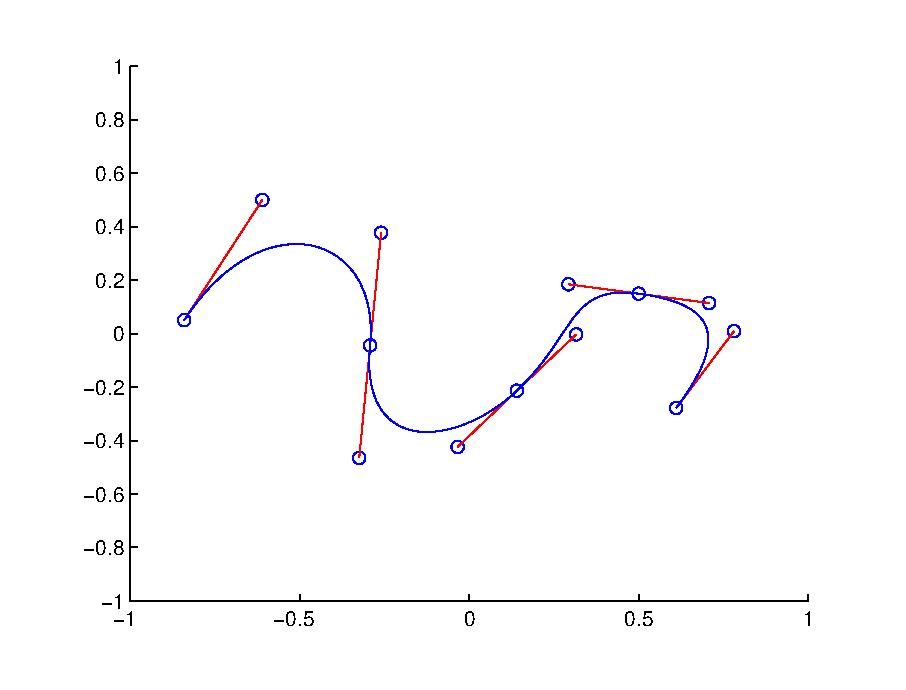
\includegraphics[height=0.495\textheight]{mynd21.eps}\\
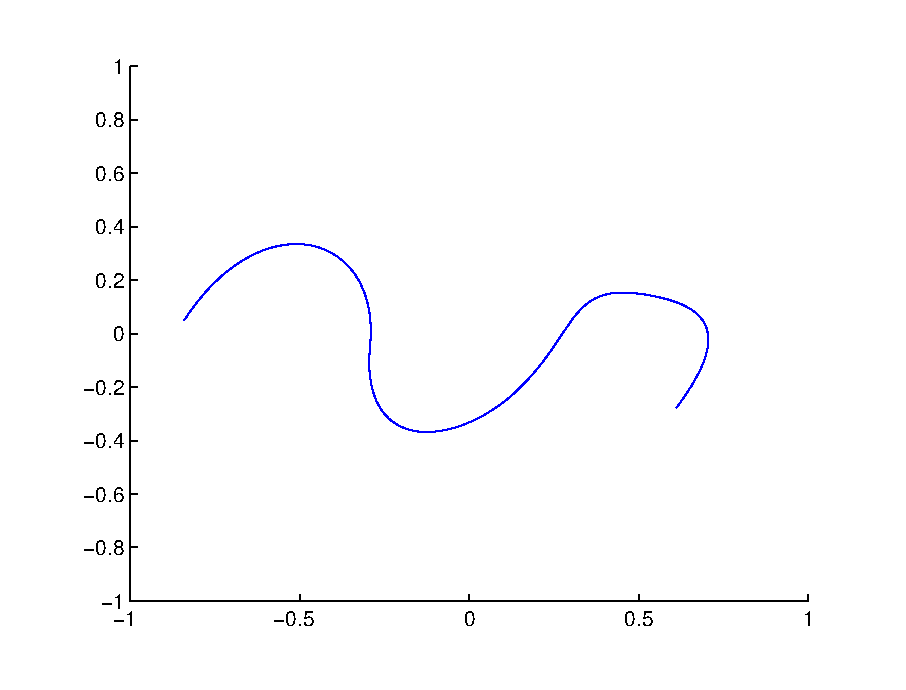
\includegraphics[height=0.495\textheight]{mynd22.eps}\\
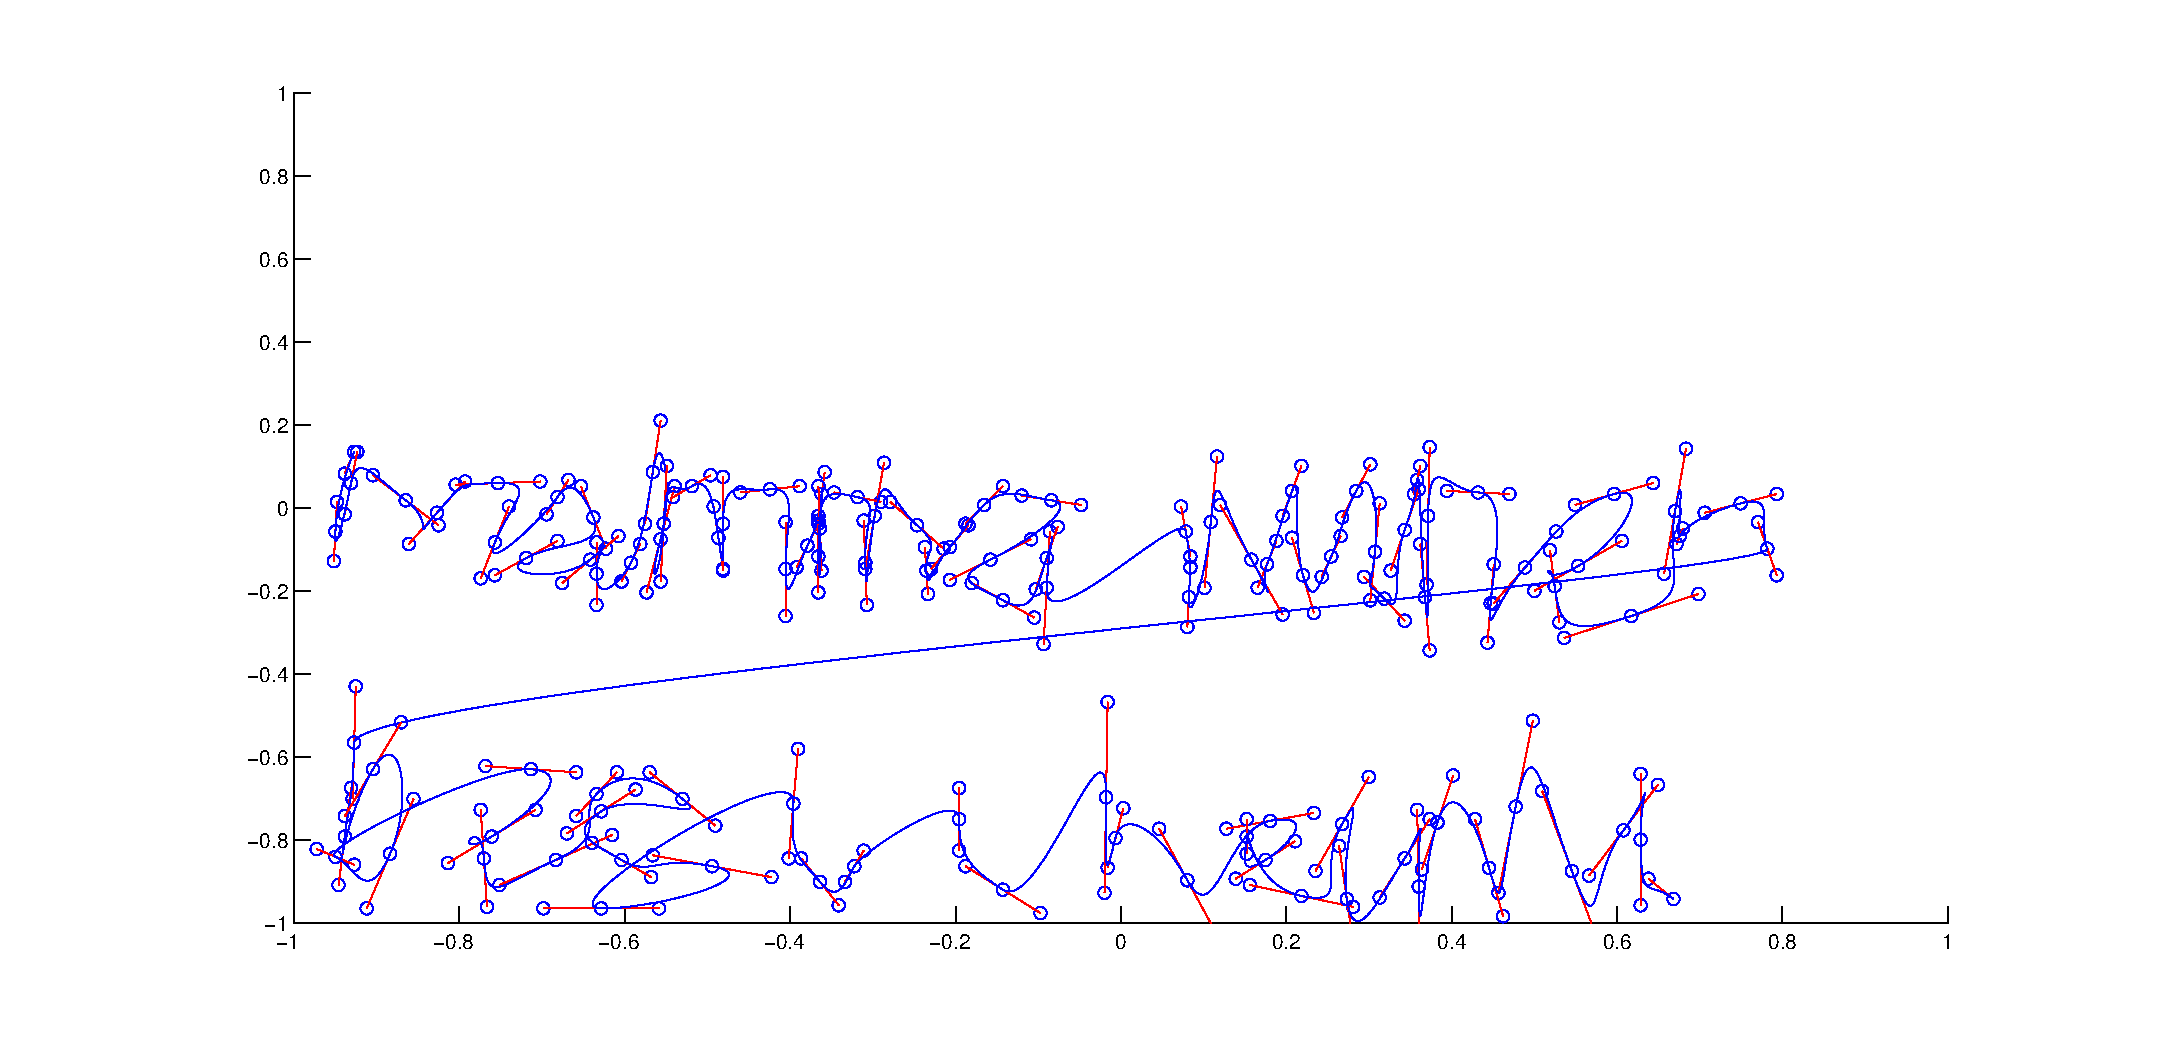
\includegraphics[width=\textwidth]{mamma1.eps}\\
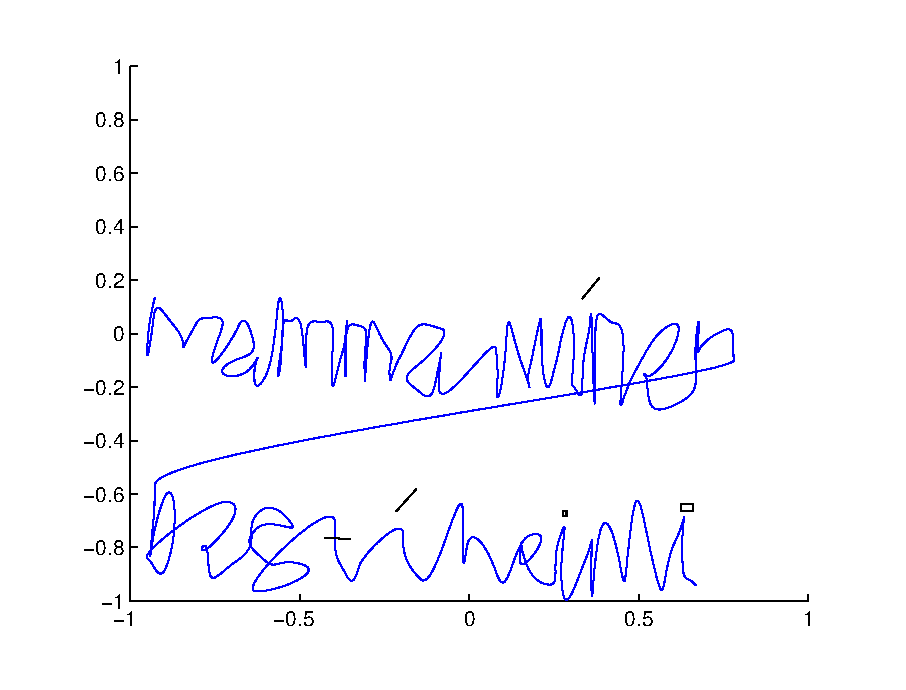
\includegraphics[height=0.495\textheight]{mamma2.eps}\\
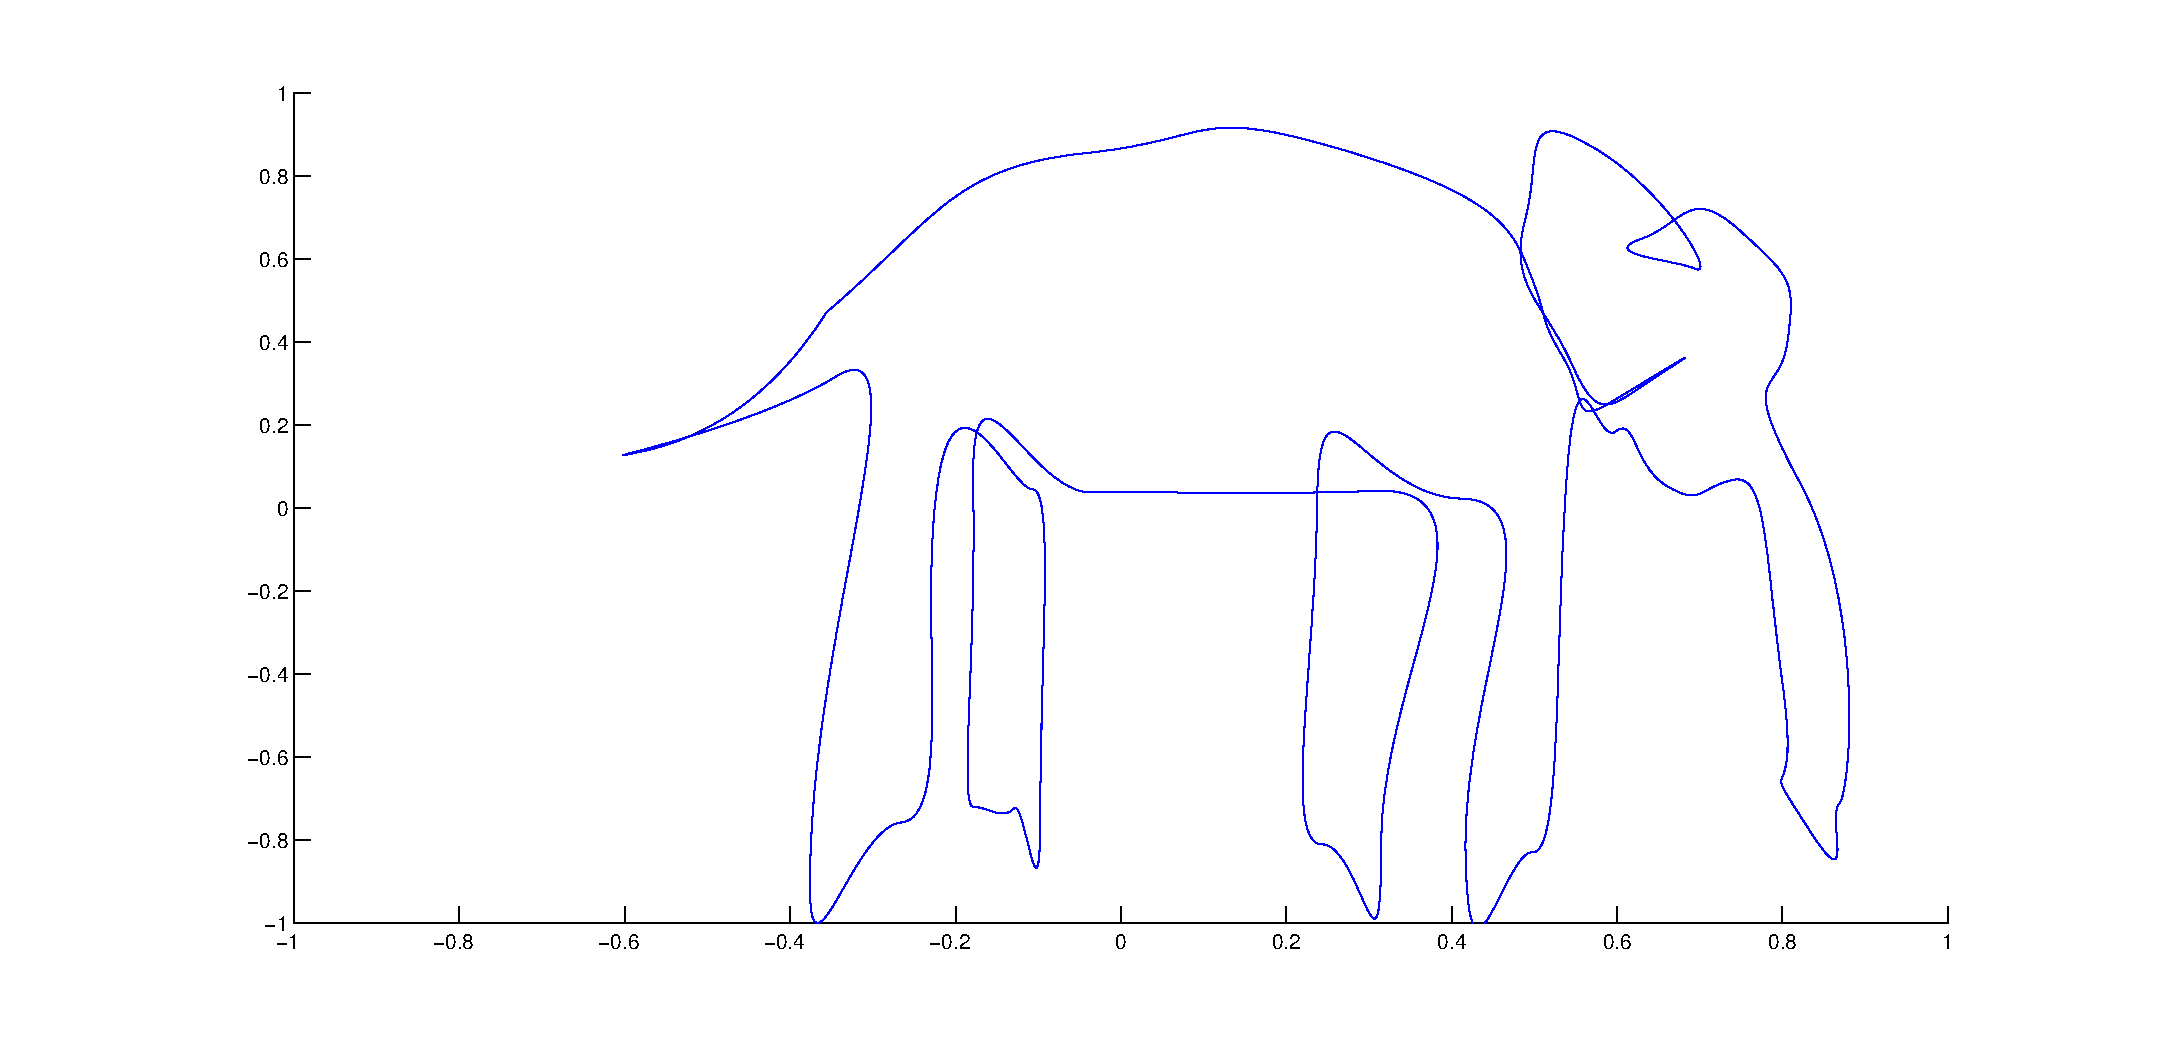
\includegraphics[width=\textwidth]{fill.eps}
hér mætti leyfa notenda að rjúfa ferilin með það er að vera með punkta sem ekki væri teiknað á milli 
Auk þess væri mjög sniðugt að geta hreyft punktana eftir að þeir hafa verið settir inn til að laga ferilin til
%Hér á að hafa inni fullt af myndarunki
\section{Nálgun á afleiðum,heildu, stiglum og Hessefylkjum}
\subsection{Almenn útgiskun}
\lstinputlisting[inputencoding=utf8]{extrapolation.m}

\subsection{Richardson}
Prófun fyrir f'(0):
Úr extrapolation kom:
\begin{lstlisting}
  function r = R(f,a,h)
      r = (f(a+h) + f(a-h))/(2*h);
  end

  >>[X,mat1,mat2]=extrapolation(@(x)sin(x), 0, 0.5, 100, 1e-10)

  X = 1 

  mat1 = 2.6201e-012

  mat2 = 1.0235e-014 
\end{lstlisting}

og úr Richardson kom:
\begin{lstlisting}
  >> [X,mat1,mat2]=richardson(@(x)sin(x), 0, 0.5, 100, 1e-10)

  X = 1

  mat1 = 2.6201e-012

  mat2 = 1.0235e-014
\end{lstlisting}
Prófun fyrir f''(0):
úr extrapolate kom
\begin{lstlisting}
  function r = R(f,a,h)
    r = (f(a+h) + f(a-h) - 2*f(a))/(h*h);
  end

  >> [X,mat1,mat2]=extrapolation(@(x)sin(x), 0, 0.5, 100, 1e-10)

  X = 0

  mat1 = 0

  mat2 = 0
\end{lstlisting}

Þar sem Richardson reiknar bara f', þannig að skiptum út fyrir cos(x) = sin'(x) til þess að prófa, en það gaf:
\begin{lstlisting}
  >> [X,mat1,mat2]=richardson(@(x)cos(x), 0, 0.5, 100, 1e-10)

  X = 0

  mat1 = 0

  mat2 = 0
\end{lstlisting}

\subsection{Romberg}
R fallið:
\begin{lstlisting}
function r = R(f,a,h,n)
    r=0;
    for i=0:n
        r = r + h*f(a+i*h);
    end
    r = r - h/2*(f(a) + f(a+n*h));
end
\end{lstlisting}
Útkoma
Keyrsla með $\sin(x)$
\begin{lstlisting}
>> [X,mat1,mat2]=extrapolation(@(x) sin(x),0,pi/2,100,1e-10)
X = 1.0000
mat1 = 1.9832e-012
mat2 = 1.9368e-015
\end{lstlisting}  
Annað dæmi með $e^x$
\begin{lstlisting}
>> [X,mat1,mat2]=extrapolation(@(x) exp(x),0,1,100,1e-10)
X = 1.7183
mat1 = 3.2863e-014
mat2 = 3.2124e-017
\end{lstlisting}

\subsection{Nálgun á stiglum}
\begin{lstlisting}
function r = R(f,a,h)
    r=[(f(a+h*[1 0]) - f(a-h*[1 0]))/(2*h);(f(a+h*[0 1]) - f(a-h*[0 1]))/(2*h)];
end
\end{lstlisting}

Keyrsla með $f(x) = x^2_1 - x^2_2$ og punktinn (1,1)
\begin{lstlisting}
>> [X,mat1,mat2]=extrapolation(@(x) x(1)^2 - x(2)^2,[1 1],1,100,1e-10)
X(:,:,1) = 2
X(:,:,2) = -2
mat1 = 0
mat2 = 0
\end{lstlisting}

Annað dæmi með $sin(x_1)*cos(x_2)$:
\begin{lstlisting}
>> [X,mat1,mat2]=extrapolation(@(x) sin(x(1))*cos(x(2)),[1 1],1,100,1e-10)
X(:,:,1) = 0.2919
X(:,:,2) = -0.7081
mat1 = 1.7925e-014
mat2 = 1.7522e-017 
\end{lstlisting}
\subsection{Nálgun á Hessefylkjum}
\vspace{20 mm}
Að skýrsluni unnu :
\hspace{0.5cm} \makebox[1.5in]{\hrulefill}
\hspace{0.5cm} \makebox[1.5in]{\hrulefill}
\hspace{0.5cm} \makebox[1.5in]{\hrulefill}
\end{document}
